Para este clasificador consideramos un enfoque parecido al de árbol de decisión, a fin de limitar las pruebas necesarias para conseguir los mejores hiper-parámetros, primero realizamos tests variando la cantidad de vecinos,k, considerados y calculando f0.5 para cross validation de 10 folds. Obteniendo los resultados de la figura ~\ref{fig:knn_f05_en_funcion_vecinos}.
Luego para los valores de k que presentaron mejores resultados ejecutamos un grid search considerando lo siguientes hiper-parámetros. 
\begin{figure}[H]
    \centering
        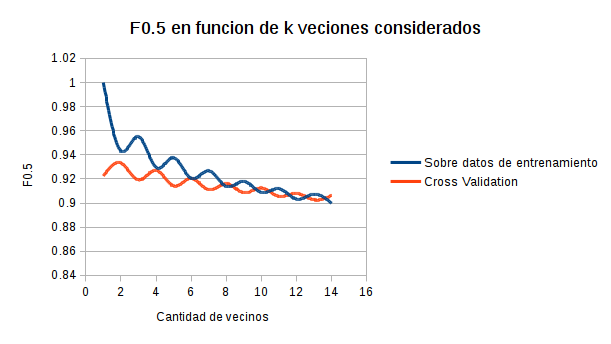
\includegraphics[width=\textwidth]{plots/knn_f05_en_funcion_vecinos.png}
        \caption{f0.5 en funcíon de k vecinos considerados}
        \label{fig:knn_f05_en_funcion_vecinos}
\end{figure}
    Se consideraron los siguiente atributos ademas de la cantidad de vecinos previamente seleccionadas para el grid search:
 \begin{enumerate}
\item \textit{Peso:} Este parámetro ponderar el peso de cada uno de los vecinos por por su distancia o tratarlos a todos uniformemente ignorando la distancia. En nuestro caso se obtuvieron mejores resultados considerando los vecinos uniformemente.  
\item \textit{Métrica de distancia:} Se probaron diferentes métricas de distancias, obteniendo los mejores resultados con la distancia manhattan en la cual la distancia entre dos puntos es la suma de las diferencias absolutas de sus coordenadas.
\end{enumerate}
